\documentclass{scrartcl}
\usepackage{amsmath,amssymb,ulem,qtree,verbatim}
\usepackage{tikz}
\usetikzlibrary{trees,arrows,automata}
\setkomafont{disposition}{\normalfont\bfseries}

\title{Toy Design Problem}
\subtitle{Foundations of Computer Science - Final Assignment}
\author{Kenny Roffo}

\begin{document}

\maketitle

The states of the following machines represent which direction the levers of the
toy are facing, in order from left to right. This means a state of LRL
represents the Levers 1 and 3 being oriented left, and Lever 2 being oriented
right. Since some of these physical states can be achieved in different manners,
if a state transition results in a final state it is labeled in the same manner,
but with an $f$ appended to the state name. The transitions themselves are
labeled 1 or 0 depending on the tube through which the ball entered the toy.
When these transitions occur, the levers' orientations are changed, thus the
state of the toy is changed.

\section{Finite State Machine}
I have designed a 5-tuple in the following manner:

\begin{align*}
M      &(Q,\Sigma,q_0,\delta,F)\\
Q      &= \{LLL,RLL,LRR,LRL,RRR,RRL,RLR,LRLf,LLRf,RRLf,LLLf,RLRf,RLLf\}\\
\Sigma &= \{0,1\}\\
q_0    &= LLL\\
F      &= \{LRLf,LLRf,RRLf,LLLf,RLRf,RLLf\}\\
\delta &: Q \times \Sigma \rightarrow Q
\end{align*}

\begin{center}
\begin{tabular} {|c|c c|}
\hline
$\delta$&$0$&$1$\\
\hline
$LLL$  & $RLL$  & $LRR$  \\
\hline
$RLL$  & $LRL$  & $RRR$  \\
\hline
$LRR$  & $RRR$  & $LRLf$ \\
\hline
$LRL$  & $RRL$  & $LLRf$ \\
\hline
$RRR$  & $LLRf$ & $RRLf$ \\
\hline
$RRL$  & $LLLf$ & $RLRf$ \\
\hline
$RLR$  & $LRR$  & $RLLf$ \\
\hline
$LRLf$ & $RRL$  & $LLRf$ \\
\hline
$LLRf$ & $RLR$  & $LLLf$ \\
\hline
$RRLf$ & $LLLf$ & $RLRf$ \\
\hline
$LLLf$ & $RLL$  & $LRR$  \\
\hline
$RLRf$ & $LRR$  & $RLLf$ \\
\hline
$RLLf$ & $LRL$  & $RRR$  \\
\hline
\end{tabular}
\end{center}
To show this DFA is minimal we start by partitioning the states into the final
and non-final states:
$$\Pi_0 :\ ^A[LLL\ RLL\ LRR\ LRL\ RRR\ RRL\ RLR]\
           ^B[LRLf\ LLRf\ RRLf\ LLLf\ RLRf\ RLLf]$$
From here we look at which sets each element maps to. For example, when the
inputs are 0 and 1, the outputs are elements of the sets $A$ and $A$ for $LLL$,
$A$ and $B$ for $LLR$, $A$ and $A$ for $RLL$, etc. Since $LLL$ and $RLL$ map to
the same sets for both inputs, they will stay together. However, $LRR$ will
branch off into a new set along with any other states which transition to
something in the set $A$ for input 0, and $B$ for input 1. Note that if elements
of $A$ have the same mappings as elements of $B$ they do not become members of
the same set at the next level of the process since they came from different
sets. This means the next step gives:
$$\Pi_1 :\ ^C[LLL\ RLL]\
           ^D[LRR\ LRL\ RLR]\
           ^E[RRR\ RRL]\
           ^F[LRLf\ LLRf\ RLRf]\
           ^G[RRLf]\
           ^H[LLLf\ RLLf]$$
We execute this process again until we find no change. Note that the $G$ set
contains one element. This is called a singleton, and is as simplified as it
can get. If after this process we only have singletons, then the machine is
already minimized.
\begin{align*}
\Pi_2 :\ &^I[LLL]\ 
           ^J[RLL]\
           ^K[LRR\ LRL]\ 
           ^L[RLR]\
           ^M[RRR]\
           ^N[RRL]\\
        &  ^O[LRLf]\
           ^P[LLRf\ RLRf]\
           ^Q[RRLf]\
           ^R[LLLf]\
           ^S[RLLf]
\end{align*}

\begin{align*}
\Pi_3 :\ &^T[LLL]\ 
           ^U[RLL]\
           ^V[LRR]\
           ^W[LRL]\ 
           ^X[RLR]\
           ^Y[RRR]\
           ^Z[RRL]\\
    &  ^\alpha[LRLf]\
        ^\beta[LLRf]\
       ^\gamma[RLRf]\
        ^\phi[RRLf]\
       ^\sigma[LLLf]\
        ^\zeta[RLLf]
\end{align*}
We see the partition has been reduced to only singleton's, so it cannot be
reduced further, and also the DFA is minimized.\pagebreak


\section{Mealy Machine}
The states and transitions in this Mealy machine are the same as for the DFA,
however there are no final states. Instead, there is an output function. The
possible outputs are $A$ and $B$, corresponding to the ball exiting through
either of these tubes.

I have designed a 6-tuple in the following manner:

\begin{align*}
M      &(Q,\Sigma,\Delta,q_0,\delta,\epsilon)\\
Q      &= \{LLL,RLL,LRR,LRL,RRR,RRL,LLR,RLR\}\\
\Delta &= \{A,B\}
\Sigma &= \{0,1\}\\
q_0    &= LLL\\
\delta &: Q \times \Sigma \rightarrow Q
\end{align*}

\begin{center}
\begin{tabular} {|c|c c|}
\hline
$\delta,\epsilon$&$0$&$1$\\
\hline
$LLL$  & $RLL,A$  & $LRR,A$  \\
\hline
$RLL$  & $LRL,A$  & $RRR,A$  \\
\hline
$LRR$  & $RRR,A$  & $LRL,B$ \\
\hline
$LRL$  & $RRL,A$  & $LLR,B$ \\
\hline
$RRR$  & $LLR,B$ & $RRL,B$ \\
\hline
$RRL$  & $LLL,B$ & $RLR,B$ \\
\hline
$LLR$ & $RLR,A$  & $LLL,B$ \\
\hline
$RLR$  & $LRR,A$  & $RLL,B$ \\
\hline
\end{tabular}
\end{center}
Now we must ensure the Mealy machine is minimized. We start with the trivial
partition where everything is in one set:
$$\Pi_0 :\ [LLL\ RLL\ LRR\ LRL\ RRR\ RRL\ LLR\ RLR]$$
Now we split this up based on the output from the different states (for example
all states which output an $A$ and $B$ for inputs 0 and 1 respectively will be
grouped together).
$$\Pi_1 :\ ^A[LLL\ RLL]\ ^B[LRR\ LRL\ LLR\ RLR]\ ^C[RRR\ RRL]$$
Finally, we continue in the same manner as for a DFA which was discussed in the
DFA section.
\begin{align*}
\Pi_2 :\ ^D[LLL]\ 
         ^E[RLL]\ 
         ^F[LRR\ LRL]\
         ^G[LLR]\ 
         ^H[RLR]\ 
         ^I[RRR]\ 
         ^J[RRL]
\end{align*}
\begin{align*}
\Pi_3 :\ ^K[LLL]\ 
         ^L[RLL]\ 
         ^M[LRR]\ 
         ^N[LRL]\
         ^O[LLR]\ 
         ^P[RLR]\ 
         ^Q[RRR]\ 
         ^R[RRL]
\end{align*}

Every set is a singleton, thus the machine is indeed minimized. 

\begin{comment}
\pagebreak
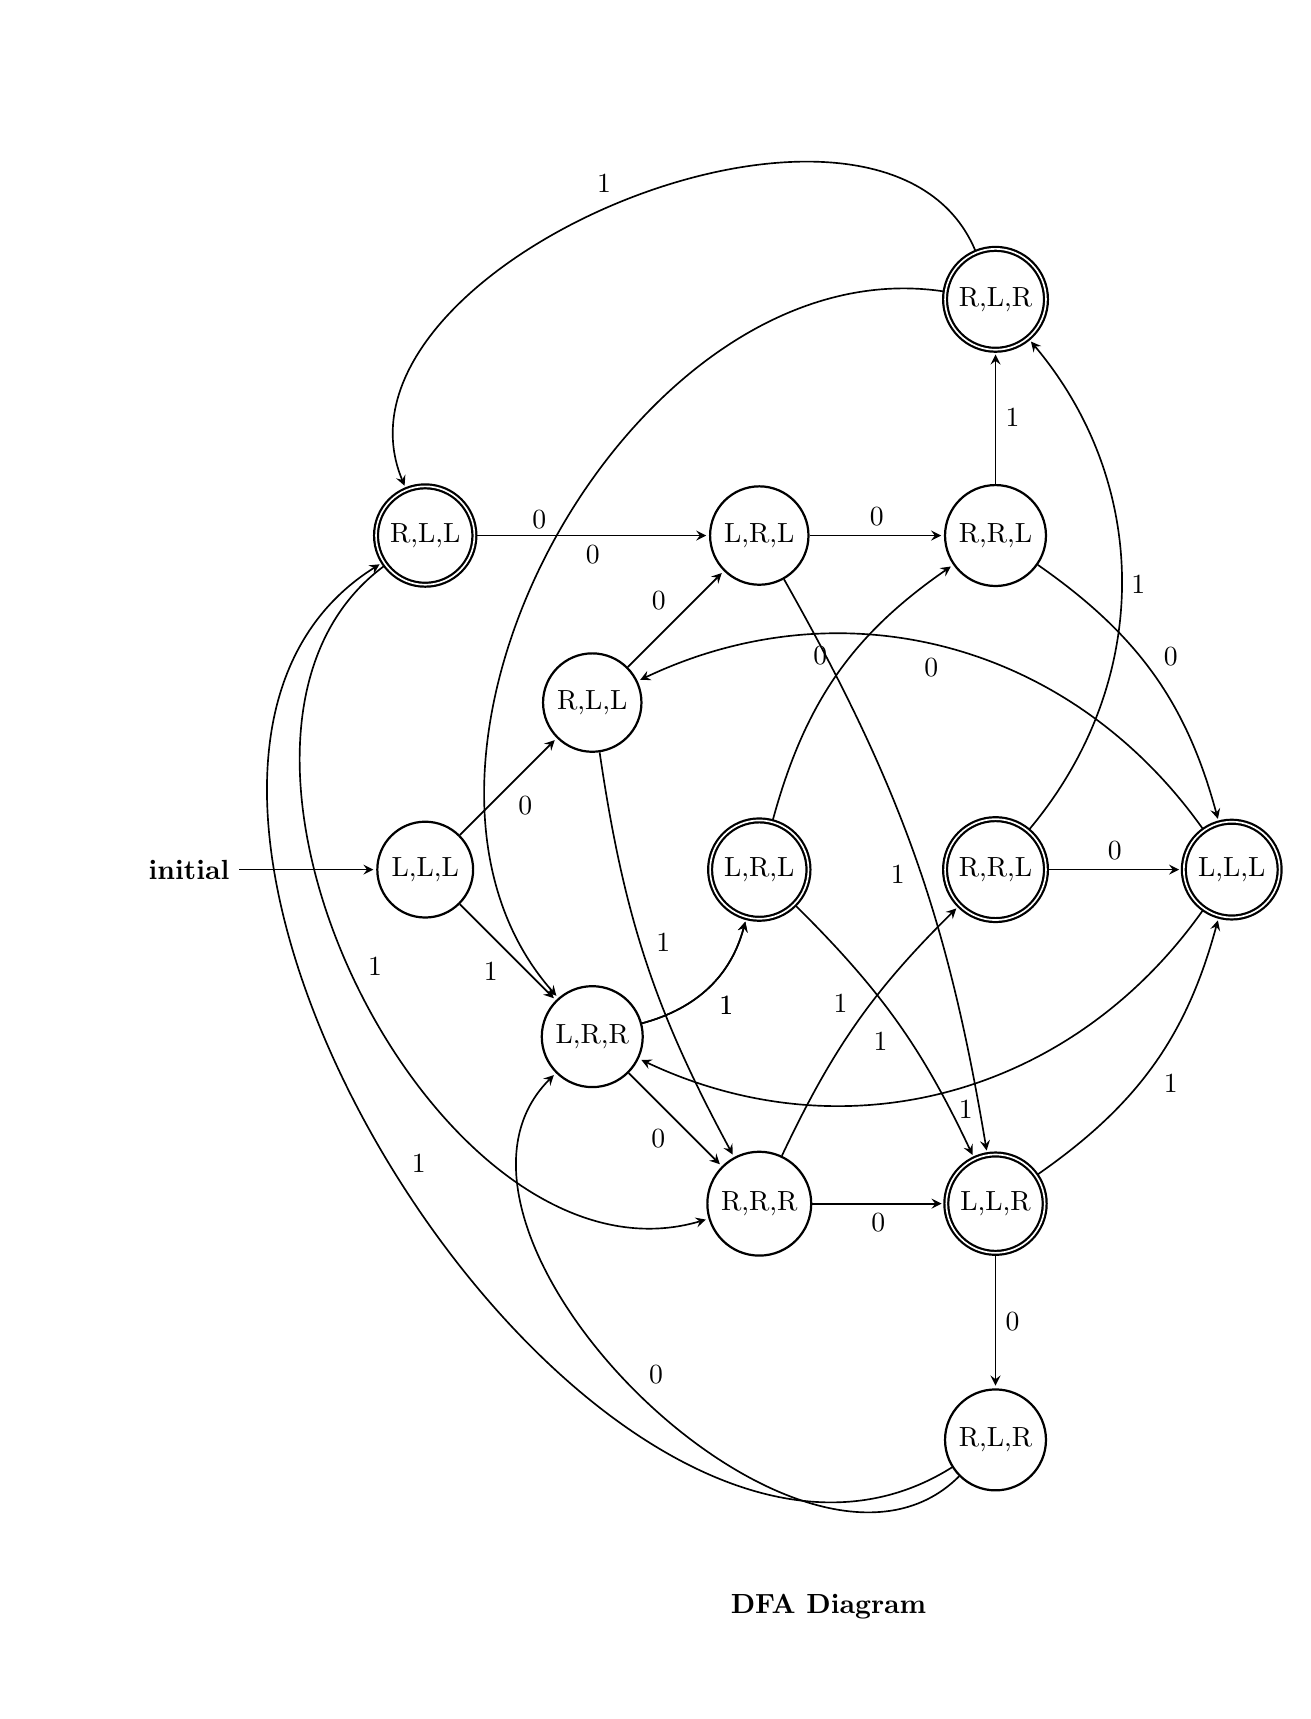
\begin{tikzpicture}
        [
            > = stealth, % arrow head style
            shorten > = 1pt, % don't touch arrow head to node
            auto,
            node distance = 3cm, % distance between nodes
            semithick % line style
        ]
        \tikzstyle{every state}=[
            draw = black,
            thick,
            fill = white,
            minimum size = 4mm
        ]

        \node (initial) {\textbf{initial}};
        \node[state] (LLL) [right of=initial] {L,L,L};
        \node[state] (RLL) [above right of=LLL] {R,L,L};
        \node[state] (LRR) [below right of=LLL] {L,R,R};
        \node[state] (LRL) [above right of=RLL] {L,R,L};
        \node[state, accepting] (LRLf) [below right of=RLL] {L,R,L};
        \node[state] (RRR) [below right of=LRR] {R,R,R};
        \node[state] (RRL) [right of=LRL] {R,R,L};
        \node[state, accepting] (RRLf) [right of=LRLf] {R,R,L};
        \node[state, accepting] (LLR) [right of=RRR] {L,L,R};
        \node[state, accepting] (RLRf) [above of=RRL] {R,L,R};
        \node[state, accepting] (LLLf) [right of=RRLf] {L,L,L};
        \node[state] (RLR) [below of=LLR] {R,L,R};
        \node[state, accepting] (RLLf) [above left of=RLL] {R,L,L};
        \node (label) [below left of=RLR] {\textbf{DFA Diagram}};        

        \path[->] (initial) edge node {} (LLL);
        \path[->, swap] (LLL) edge node {$0$} (RLL);
        \path[->, swap] (LLL) edge node {$1$} (LRR);
        \path[->] (RLL) edge node {$0$} (LRL);
        \path[->, bend right=10] (RLL) edge node {$1$} (RRR);
        \path[->, bend right=30, swap] (LRR) edge node {$1$} (LRLf);
        \path[->, swap] (LRR) edge node {$0$} (RRR);
        \path[->] (LRL) edge node {$0$} (RRL);
        \path[->, bend left=10, swap] (LRL) edge node {$1$} (LLR);
        \path[->, bend left=20] (LRLf) edge node {$0$} (RRL);
        \path[->, bend left=10, swap] (LRLf) edge node {$1$} (LLR);
        \path[->, bend left=10] (RRR) edge node {$1$} (RRLf);
        \path[->, swap] (RRR) edge node {$0$} (LLR);
        \path[->, bend right=30, swap] (LRR) edge node {$1$} (LRLf);
        \path[->, bend left=20] (RRL) edge node {$0$} (LLLf);
        \path[->, swap] (RRL) edge node {$1$} (RLRf);
        \path[->] (RRLf) edge node {$0$} (LLLf);
        \path[->, bend right=40, swap] (RRLf) edge node {$1$} (RLRf);
        \path[->] (LLR) edge node {$0$} (RLR);
        \path[->, bend right=20, swap] (LLR) edge node {$1$} (LLLf);
        \path[->, bend left=90, swap] (RLR) edge node {$0$} (LRR);
        \path[->, bend left=90, swap] (RLR) edge node {$1$} (RLLf);
        \path[->, bend right=70, swap] (RLRf) edge node {$0$} (LRR);
        \path[->, bend right=90, swap] (RLRf) edge node {$1$} (RLLf);
        \path[->, bend left=40] (LLLf) edge node {$1$} (LRR);
        \path[->, bend right=40] (LLLf) edge node {$0$} (RLL);
        \path[->,swap] (RLLf) edge node {$0$} (LRL);
        \path[->, bend right=80] (RLLf) edge node {$1$} (RRR);
          
    \end{tikzpicture}

\pagebreak
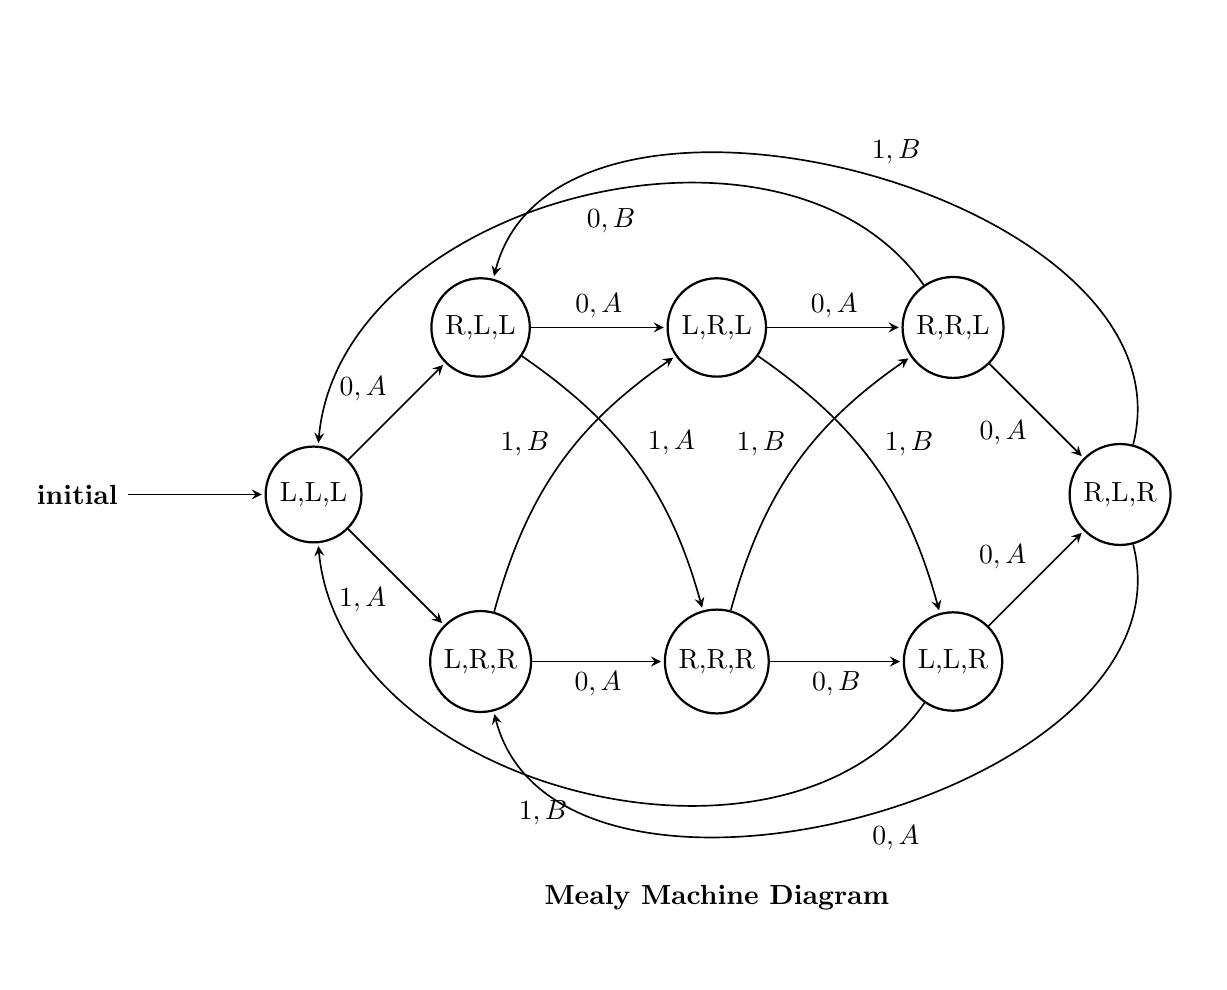
\begin{tikzpicture}
        [
            > = stealth, % arrow head style
            shorten > = 1pt, % don't touch arrow head to node
            auto,
            node distance = 3cm, % distance between nodes
            semithick % line style
        ]
        \tikzstyle{every state}=[
            draw = black,
            thick,
            fill = white,
            minimum size = 4mm
        ]

        \node (initial) {\textbf{initial}};
        \node[state] (LLL) [right of=initial] {L,L,L};
        \node[state] (RLL) [above right of=LLL] {R,L,L};
        \node[state] (LRR) [below right of=LLL] {L,R,R};
        \node[state] (LRL) [right of=RLL] {L,R,L};
        \node[state] (RRR) [right of=LRR] {R,R,R};
        \node[state] (RRL) [right of=LRL] {R,R,L};
        \node[state] (LLR) [right of=RRR] {L,L,R};
        \node[state] (RLR) [above right of=LLR] {R,L,R};
        \node (label) [below of=RRR] {\textbf{Mealy Machine Diagram}};

        \path[->] (initial) edge node {} (LLL);
        \path[->] (LLL) edge node {$0,A$} (RLL);
        \path[->, swap] (LLL) edge node {$1,A$} (LRR);
        \path[->] (RLL) edge node {$0,A$} (LRL);
        \path[->, bend left=20] (RLL) edge node {$1,A$} (RRR);
        \path[->, swap] (LRR) edge node {$0,A$} (RRR);
        \path[->, bend left=20] (LRR) edge node {$1,B$} (LRL);
        \path[->] (LRL) edge node {$0,A$} (RRL);
        \path[->, bend left=20] (LRL) edge node {$1,B$} (LLR);
        \path[->, bend left=20] (RRR) edge node {$1,B$} (RRL);
        \path[->, swap] (RRR) edge node {$0,B$} (LLR);
        \path[->] (LLR) edge node {$0,A$} (RLR);
        \path[->, swap] (RRL) edge node {$0,A$} (RLR);
        \path[->, bend left=90] (RLR) edge node {$0,A$} (LRR);
        \path[->, bend right=90, swap] (RLR) edge node {$1,B$} (RLL);
        \path[->, bend right=70] (RRL) edge node {$0,B$} (LLL);
        \path[->, bend left=70] (LLR) edge node {$1,B$} (LLL);
    \end{tikzpicture}
\end{comment}
\end{document}
